\section{Cực trị}
\subsection{Kiến thức cần nhớ}
\begin{khung}
	\subsubsection{Cực trị}
	\begin{itemize}
		\item Số cực trị của hàm số là số nghiệm đơn hoặc bội lẻ của phương trình $f'(x)=0$.
		\item Do đó, để tìm số điều kiện để hàm số có $n$ cực trị thì ta đi tìm điều kiện của $m$  để phương trình $f'(x)=0$ có $n$ nghiệm bội lẻ.
		\item Ta thường phân li $m$ của phương trình về dạng $m=g(x)$ và dùng công cụ khảo sát hàm số tìm điều kiện $m$ thỏa mãn bài toán.
		\item PTĐT qua các điểm cực trị của hàm số bậc ba $y=ax^3+bx^2+cx+d,(a\ne 0 )$ là $$g(x)=\left( \dfrac{2c}{3}-\dfrac{2{{b}^{2}}}{9a} \right)x+d-\dfrac{bc}{9a} $$
		hoặc  $$ g( x )=y-\frac{{y}'.{y}''}{18a}$$
		 hoặc  $$g( x )=y-\frac{{y}'.{y}''}{3{y}'''}$$
		\item Giả sử hàm số $y=a{{x}^{4}}+b{{x}^{2}}+c$ có ba cực trị, thì tọa độ ba điểm cực trị là:
		$$A(0;c),B\left( -\sqrt{-\frac{b}{2a}};-\frac{\Delta }{4a} \right),C\left( \sqrt{-\frac{b}{2a}};-\frac{\Delta }{4a} \right)$$
		\end{itemize}
\end{khung}
\subsection{Bài tập mẫu}
\Opensolutionfile{ans}[ans/ANS-DANG-1]
\begin{khung}
	\begin{vd}[Đề minh họa BGD 2022-2023]%[Thái Văn Sang, ĐMH]%[2D1G2-6] %Câu 1
		Có bao nhiêu số nguyên $m$ để hàm số $y=x^3-3x^2-mx+4$ có hai điểm cực trị thuộc khoảng $(-3;3)$?
		\choice
		{$13$}
		{$10$}
		{$12$}
		{\True $11$}
		\loigiai{
			Ta có $$y'=3x^2-6x-m$$
			Hàm số có hai điểm cực trị thuộc khoảng $(-3;3)$ khi và chỉ khi phương trình $y'=0$ có hai nghiệm phân biệt $x_1,x_2 \in (-3;3)$.
			$$\Leftrightarrow 3x^2-6x-m=0$$ có hai nghiệm phân biệt $x_1,x_2 \in (-3;3).$
			$$\Leftrightarrow m=3x^2-6x$$ có hai nghiệm phân biệt $x_1,x_2 \in (-3;3)$.\\
				Xét hàm số $$f(x)=3x^2-6x.$$
			Ta có $$f'(x)=6x-6; f'(x)=0 \Leftrightarrow x=1.$$
			Bảng biến thiên
		\begin{center}
			\begin{tikzpicture}
			\tkzTabInit[nocadre,lgt=1.5,espcl=2,deltacl=.5]
			{$x$/0.7, $f’(x)$/0.7, $f(x)$/2}
			{$-3$,$1$,$3$}
			\tkzTabLine{,-,0,+,}
			\tkzTabVar{+/$45$, -/$-3$, +/$9$}
			\end{tikzpicture}
		\end{center}
			Dựa vào bảng biến thiên ta có $-3<m<9$.\\
			Vậy $m \in \big\{-2;-1;0;\ldots;8\big\}$.
		}

	\end{vd}
\end{khung}
\subsection{Bài tập tương tự và phát triển}
\begin{ex}%[Thái Văn Sang, ĐMH]%%[2D1G2-5]
	Tính tổng các giá trị nguyên dương của tham số $m$ để hàm số $y=x^4+(m-5)x^2+5$ có $3$ điểm cực trị.
	\choice
	{$4$}
	{\True $10$}
	{$15$}
	{$24$}
	\loigiai{
	Ta có $$y'=4x^3+2(m-5)x$$
		$$\Rightarrow y'=0 \Leftrightarrow 2x(2x^2+m-5)=0$$
		$$ \Leftrightarrow \hoac{&2x=0\\&2x^2+m-5=0}$$
		$$ \Leftrightarrow \hoac{&x=0\\&2x^2=-m+5 \quad (1).}$$
		Hàm số $y=x^4+(m-5)x^2+5$ có $3$ điểm cực trị khi và chỉ khi phương trình $(1)$ có $2$ nghiệm phân biệt khác $0$ $$\Leftrightarrow \heva{&-m+5>0\\&2 \cdot 0^2+m-5 \ne 0} \Leftrightarrow \heva{&m<5\\&m \ne 5} \Leftrightarrow m<5.$$
		$$\Rightarrow m \in \big\{1;2;3;4 \big\}.$$
		Vậy tổng các giá trị nguyên dương của tham số $m$ bằng $10$.
	}
\end{ex}
\begin{ex}%Câu 3%[Thái Văn Sang, ĐMH]%[2D1G2-6]
	Tìm tổng tất cả các giá trị nguyên của tham số $m$ trên $(-10;10)$ để đồ thị hàm số $y=x^3+x^2+mx-1$ có điểm cực tiểu của nằm bên phải trục tung.
	\choice
	{$0$}
	{$-55$}
	{\True $-45$}
	{$45$}
	\loigiai{
		Ta có $$y'=3x^2+2x+m$$
		Để hàm số có cực tiểu, tức hàm số có hai cực trị thì phương trình $y'=0$ có hai nghiệm phân biệt\\
		Điều này tương đương với phương trình $3x^2+2x+m=0 \quad (1)$ có hai nghiệm phân biệt; $(1)$ có hai nghiệm phân biệt khi và chỉ khi $${\Delta}'=1-3m>0 \Leftrightarrow m<\dfrac{1}{3}.$$
		Khi đó $(1)$ có hai nghiệm phân biệt $x_{\text{CĐ}}$, $x_{\text{CT}}$ là hoành độ hai điểm cực trị. Theo định lí Viet ta có $$\heva{&x_{\text{CĐ}}+x_{\text{CT}}=-\dfrac{2}{3}<0 \quad(2)\\&x_{\text{CĐ}} \cdot x_{\text{CT}}=\dfrac{m}{3} \quad (3)},$$ trong đó $$x_{\text{CĐ}} <x_{\text{CT}}$$ vì hệ số của $x^3$ lớn hơn $0$.\\
		Để cực tiểu của đồ thị hàm số nằm bên phải trục tung thì phải có: $$x_{\text{CT}}>0,$$ kết hợp $(2)$ và $(3)$ suy ra $(1)$ có hai nghiệm trái dấu $$\Leftrightarrow x_{\text{CĐ}} \cdot x_{\text{CT}}=\dfrac{m}{3}<0 \Leftrightarrow m<0.$$
		Mà $m<\dfrac{1}{3}, m \in (-10;10),m \in \mathbb{Z}$ nên $m \in \big\{-9;-8;-7;\ldots;-1\big\}$.\\
		Vậy tổng tất cả các giá trị của tham số $m$ thỏa mãn YCBT là: $-45$.
	}
\end{ex}

\begin{ex}%Câu 3%[Thái Văn Sang, ĐMH]%[2D1G2-6]]
	Có bao nhiêu giá trị thực của tham số $m$ để đồ thị hàm số $y=\dfrac{x^3}{3}-(5m^2-3m-1)x^2+(2m+1)x+1$ có hai điểm cực trị $A,B$ sao cho $A,B$ cách đều đường thẳng $\Delta \colon x-1=0$?
	\choice
	{\True $1$}
	{$0$}
	{$2$}
	{$3$}
	\loigiai{
		Tập xác định: $\mathscr{D}=\mathbb{R}$.\\
		Đạo hàm: $$y'=x^2-2(5m^2-3m-1)x+2m+1$$
		$$y'=0 \Leftrightarrow x^2-2(5m^2-3m-1)x+2m+1=0 \quad(1)$$
		Đồ thị hàm số có hai điểm cực trị $A,B$ khi và chỉ khi $(1)$ có hai nghiệm phân biệt.\\
		Khi đó: 
		$$\Delta '>0 \Leftrightarrow (5m^2-3m-1)^2-(2m+1)>0 \quad(*)$$
		Với điều kiện $(*)$, phương trình $(1)$ có hai nghiệm phân biệt $x_1,x_2$ thỏa mãn
		$$\heva{&x_1+x_2=2(5m^2-3m-1)\\&x_1 \cdot x_2=2m+1.} \quad(**)$$
		Giả sử tọa độ hai điểm cực trị 
		$$A\left( x_1;\dfrac{x_1^3}{3}-(5m^2-3m-1)x_1^2+(2m+1)x_1+1 \right)$$
		$$B\left( x_2;\dfrac{x_2^3}{3}-(5m^2-3m-1)x_2^2+(2m+1)x_2+1 \right).$$
		Theo giả thiết, hai điểm cực trị cách đều đường thẳng $\Delta \colon x-1=0$ nên ta có
		$$\mathrm{d}\left( A, \Delta \right)=\mathrm{d}\left( B, \Delta \right) \Leftrightarrow |x_1-1|=|x_2-1|\Leftrightarrow x_1+x_2=2.$$
		Kết hợp với hệ $(**)$ suy ra
		$$2(5m^2-3m-1)=2 \Leftrightarrow 5m^2-3m-2=0 \Leftrightarrow \hoac{&m=1\\&m=-\dfrac{2}{5}.}$$\
		Kiểm tra với điều kiện $(*)$ thấy $m=-\dfrac{2}{5}$ thỏa mãn.\\
		Vậy có $1$ giá trị thực của tham số $m$ thỏa mãn yêu cầu bài toán.
	}
\end{ex}
\begin{ex}%Câu 3%[Thái Văn Sang, ĐMH]%[2D1G2-6]]
	Tổng tất cả các giá trị của m để đồ thị hàm số $y=x^3+3x^2+m-1$ có hai điểm cực trị $A, B$ sao cho tam giác $OAB$ vuông tại $O$.
	\choice
	{$4$}
	{\True $-3$}
	{$-2$}
	{$2$}
	\loigiai{
		Ta có 
		$$y'=3x^2+6x=0 \Rightarrow \hoac{&x=0;y=m-1\\&x=-2;y=3+m} \Rightarrow A(0;m-1),B(-2;m+3).$$
		Tam giác $\triangle OAB $ vuông tại $0$ khi và chỉ khi $$ \overrightarrow{OA} \cdot \overrightarrow{OB}=0 \Leftrightarrow m=1 \vee m=-3.$$
		Kiểm tra lại $m=1 \Rightarrow A(0;0) \equiv O$ nên loại $m=1$.\\
		 Vậy chỉ có $m=-3$.
	}
\end{ex}


\begin{ex}%Câu 3%[Thái Văn Sang, ĐMH]%[2D1G2-6]]
	Cho hàm số $y=-x^3-3x^2+4$. Biết rằng có hai giá trị $m_1$, $m_2$ của tham số $m$ để đường thẳng đi qua hai điểm cực trị của đồ thị hàm số tiếp xúc với đường tròn $(C) \colon (x-m)^2+(y-m-1)^2=5$. Tính tổng $m_1+m_2$.
	\choice
	{\True $m_1+m_2=-6$}
	{$m_1+m_2=10$}
	{$m_1+m_2=6$}
	{$m_1+m_2=0$}
	\loigiai{
		Ta có 
		$$ y'=-3x^2-6x$$
		và 
		$$y=\left( \dfrac{x}{3}+\dfrac{1}{3} \right)y'+2x+4,$$
		 suy ra PTĐT đi qua hai điểm cực trị của đồ thị hàm số là 
		 $$y=2x+4 \Leftrightarrow 2x-y+4=0, \left( \Delta \right).$$
		Đường tròn $$(C) \colon (x-m)^2+(y-m-1)^2=5$$
		 có tâm $I(m;m+1)$ và bán kính $R=\sqrt{5}$.\\
		Đường thẳng $\left( \Delta \right)$ tiếp xúc với đường tròn $(C)$ khi và chỉ khi 
			$$\mathrm{d}\left( I,\left( \Delta \right) \right)=R \Leftrightarrow \dfrac{|2m-m-1+4|}{\sqrt{5}}=\sqrt{5} \Leftrightarrow |m+3|=5 \Leftrightarrow \hoac{&m=2\\&m=-8.}$$
		 Vậy $m_1+m_2=-6.$
	}
\end{ex}
\begin{ex}%Câu 3%[Thái Văn Sang, ĐMH]%[2D1G2-5]]
	Tìm tất cả các giá trị của tham số $m$ sao cho đồ thị hàm số $y=x^4+(m+1)x^2-2m-1$ có ba điểm cực trị là ba đỉnh của một tam giác có một góc bằng $120^{\circ}$.
	\choice
	{$m<-1$}
	{$m=-1-\dfrac{2}{\sqrt[3]{3}}$, $m=-1$}
	{$m=-\dfrac{1}{\sqrt[3]{3}}$}
	{\True $m=-1-\dfrac{2}{\sqrt[3]{3}}$}
	\loigiai{
		Tập xác định: $\mathscr{D}=\mathbb{R}.$\\
		Hàm số có ba điểm cực trị $\Leftrightarrow m+1<0$ $\Leftrightarrow m<-1$.\\
		Khi đó 
		$$A(0;-2m-1), B\left( -\sqrt{\dfrac{-m-1}{2}};-\dfrac{(m+1)^2}{4}-2m-1 \right), C\left( \sqrt{\dfrac{-m-1}{2}};-\dfrac{(m+1)^2}{4}-2m-1 \right)$$
		 và 
		 $$H\left( 0;-\dfrac{(m+1)^2}{4}-2m-1 \right) (H \text{ là trung điểm } BC).$$
		Do tam giác $ABC$ cân tại $A$ $\Rightarrow \widehat{A}=120^{\circ}$.\\
		Ta có
		\allowdisplaybreaks
		\begin{eqnarray*}
			 BH&=&AH\tan 60^{\circ}\\
		\Leftrightarrow  \dfrac{(m+1)^2}{4} \cdot \sqrt{3}&=&\sqrt{-\dfrac{m+1}{2}}\\ \Leftrightarrow  \dfrac{3(m+1)^4}{16}&=&-\dfrac{m+1}{2}\\ \Leftrightarrow  3(m+1)^3&=&-8\\ \Leftrightarrow  m&=&-1-\dfrac{2}{\sqrt[3]{3}}\quad(\text{nhận}).
		\end{eqnarray*}
	}
\end{ex}
\begin{ex}%%Câu 3%[Thái Văn Sang, ĐMH]%[2D1G2-5]]
	Cho biết đồ thị hàm số $y=x^4-2mx^2-2m^2+m^4$ có 3 điểm cực trị $A$, $B$, $C$ cùng với điểm $D(0;-3)$ là 4 đỉnh của một hình thoi. Gọi $S$ là tổng các giá trị của $m$ thỏa mãn đề bài thì $S$ thuộc khoảng nào sau đây?
	\choice
	{$S \in \left( 0;\dfrac{5}{2} \right)$}
	{$S \in \left( \dfrac{9}{2};6 \right)$}
	{$S \in \left( 1;\dfrac{5}{2} \right)$}
	{\True $S \in (2;4)$}
	\loigiai{
		Ta có $$y=x^4-2mx^2-2m^2+m^4$$ có 3 điểm cực trị $A$, $B$, $C$
		$$y'=4x^3-4mx=4x(x^2-m)$$ có 3 nghiệm phân biệt suy ra $m>0.$\\
		Không làm mất tính tổng quát giả sử
		$$A(0;m^4-2m^2);B\left( \sqrt{m};m^4-3m^2 \right);C\left( -\sqrt{m};m^4-3m^2 \right);$$
		Gọi $I=AD \cap BC$ ($A,D \in Oy$)\\
		$I$ là trung điểm của $BC$ $\Rightarrow I(0;m^4-3m^2).$\\
		$I$ là trung điểm của $AD$ $\Rightarrow I\left( 0;\dfrac{m^4-2m^2-3}{2} \right).$\\
		Đồng nhất ta có 
		$$\dfrac{m^4-2m^2-3}{2}=m^4-3m^2 \Leftrightarrow m^4-4m^2+3=0 \Leftrightarrow \hoac{&m=\pm 1\\&m=\pm \sqrt{3}.}$$
		Kết hợp với đk ta có $$m=1,m=\sqrt{3} \Rightarrow S=1+\sqrt{3}.$$
		Vậy $S \in (2;4)$.
	}
\end{ex}

\begin{ex}%Câu 3%[Thái Văn Sang, ĐMH]%[2D1G2-5]
	Cho hàm số $y=x^4+2(m-4)x^2+m+5$ có đồ thị $(C_m)$. Tìm $m$ để $(C_m)$ có ba điểm cực trị tạo thành một tam giác nhận gốc tọa độ $O$ làm trọng tâm.
	\choice
	{$m=4$}
	{$m=\dfrac{17}{2}$}
	{$m=1$ hoặc $m=\dfrac{17}{2}$}
	{\True $m=1$}
	\loigiai{
		Ta có 
		$$y'=4x^3+4(m-4)x;$$
		$$ y'=0 \Leftrightarrow \hoac{&x=0\\&x^2=4-m.}$$
		Để hàm số có ba điểm cực trị $\Leftrightarrow m<4$. Khi đó các điểm cực trị của $(C_m)$ là
	$$ A(0;m+5), B\left( \sqrt{4-m};m+5-(m-4)^2 \right), C\left( -\sqrt{4-m};m+5-(m-4)^2 \right).$$
					
		Do $O$ là trọng tâm tam giác $ABC$ nên 
		$$ 3(m+5)=2(m-4)^2 \Leftrightarrow \hoac{&m=1\\&m=\dfrac{17}{2}.}$$
		Do $m<4$ nên $m=1$.
	}
\end{ex}

\begin{ex}%Câu 3%[Thái Văn Sang, ĐMH]%[2D1G2-5]
	Cho hàm số $y=x^4-2mx^2+3m$ $(C_m)$. Có bao nhiêu giá trị nguyên của tham số $m$ để $(C_m)$ có ba điểm cực trị và khoảng cách giữa hai điểm cực tiểu của $(C_m)$ nhỏ hơn $4$?
	\choice
	{$3$}
	{\True  Vô số}
	{$4$}
	{$1$}
	\loigiai{
		Ta có $y=x^4-2mx^2+3m$;\\
		 $y'=4x^3-4mx$;
$$y'=0 \Leftrightarrow \hoac{&x=0\\&x^2-m=0.}$$
		Hàm số có $3$ cực trị khi $m>0$, khi đó khoảng cách hai điểm cực tiểu của $(C_m)$ là $2\sqrt{m}$.\\
		Theo giả thiết, ta có 
		$$2\sqrt{m}<4 \Leftrightarrow m<4.$$
		Vậy các giá trị nguyên của $m$ thỏa yêu cầu bài toán là $m \in \big\{3;2;1;0;-1; \cdots\big\}$.
	}
\end{ex}
\begin{ex}%[Thái Văn Sang, ĐMH]%[2D1G2-5]
	Biết đồ thị hai hàm số $y=x^4-2x^2+2$ và $y=mx^4+nx^2-1$ có chung ít nhất một điểm cực trị. Giá trị của biểu thức $2m+3n$ bằng
	\choice
	{$11$}
	{$10$}
	{\True $8$}
	{$9$}
	\loigiai{
		Ta có\\
		Đồ thị hàm số $$y=x^4-2x^2+2 (C_1)$$ có ba điểm cực trị là $$A(0;2),B(1;1),C(-1;1).$$
		Đồ thị hàm số $$y=mx^4+nx^2-1 (C_2)$$ có 1 điểm cực trị là $D(0;-1)$ không trùng với ba điểm cực trị của $(C_1)$, kết hợp đề bài ta suy ra $(C_2)$ có ba điểm cực trị hay $m \cdot n<0$.\\
		$(C_2)$ có thêm hai điểm cực trị nữa là
		$$E\left( \sqrt{-\dfrac{n}{2m}};-\dfrac{n^2}{4m}-1 \right), F\left( -\sqrt{-\dfrac{n}{2m}};-\dfrac{n^2}{4m}-1 \right).$$
		Từ giả thiết ta suy ra $E \equiv B$ hay
		$$\heva{&\sqrt{-\dfrac{n}{2m}}=1\\&-\dfrac{n^2}{4m}-1=1} \Rightarrow \heva{&m=-2\\&n=4.}$$
	 		Do đó $2m+3n=8$.
	}
\end{ex}

\begin{ex}%[Thái Văn Sang, ĐMH]%[2D1G2-5]
	Cho hàm số $y=x^4-2mx^2+1-m$. Tìm tất cả các giá trị thực của tham số $m$ để đồ thị hàm số có ba điểm cực trị tạo thành một tam giác nhận gốc tọa độ $O$ làm trực tâm.
	\choice
	{$m=-1$}
	{$m=2$}
	{$m=0$}
	{\True $m=1$}
	\loigiai{
		Ta có $$y'=4x^3-4mx=0 \Leftrightarrow 4x(x^2-m)=0 \Leftrightarrow \hoac{&x=0\\&x^2=m.}$$
		Hàm số có 3 điểm cực trị khi và chỉ khi $m>0$.\\
		Khi đó gọi 
$$ A(0;1-m), B\left( \sqrt{m};-m^2+1-m \right), C\left( -\sqrt{m};-m^2+1-m \right)$$
		là các điểm cực trị của đồ thị hàm số.\\
		Ta có 
	$$\overrightarrow{OA}=(0;1-m), \overrightarrow{BC}=\left( -2\sqrt{m};0 \right), \overrightarrow{OB}=\left( \sqrt{m};-m^2+1-m \right) \text{ và } \overrightarrow{AC}=\left( -\sqrt{m};-m^2 \right).$$
	
		Gốc $O$ là trực tâm của tam giác $ABC$ thì
	$$\heva{&\overrightarrow{OA} \cdot \overrightarrow{BC}=0\\&\overrightarrow{OB} \cdot \overrightarrow{AC}=0} \Leftrightarrow \heva{&-2\sqrt{m} \cdot 0+(1-m) \cdot 0=0\\&-\sqrt{m} \cdot \sqrt{m}-m^2(-m^2+1-m)=0}
	\Leftrightarrow \heva{&0=0\\&-m+m^4-m^2+m^3=0} $$
		$$	\Leftrightarrow m(m^3+m^2-m-1)=0 \Leftrightarrow \hoac{&m=0\\& m=1\\& m=-1}.$$
			Kết hợp điều kiện $m>0$ ta có $m=1$.
	}
\end{ex}

\begin{ex}%[Thái Văn Sang, ĐMH]%[2D1G2-5]
	Tìm tất cả các giá trị $m$ sao cho đồ thị hàm số $y=x^4+(m+1)x^2-2m-1$ có ba điểm cực trị là ba đỉnh của một tam giác có một góc bằng $120^{\circ}$.
	\choice
	{$m=-\dfrac{1}{\sqrt[3]{3}}$}
	{$m<-1$}
	{\True $m=-1-\dfrac{2}{\sqrt[3]{3}}$}
	{$m=-1-\dfrac{2}{\sqrt[3]{3}}$, $m=-1$}
	\loigiai{
		Ta có $y'=4x^3+2(m+1)x=2x(2x^2+m+1)$.
		$$y'=0 \Leftrightarrow \hoac{&x=0\\&2x^2=-m-1.}$$
		Hàm số có ba điểm cực trị khi và chỉ khi $y'=0$ có ba nghiệm phân biệt
$$\Leftrightarrow m+1<0 \Leftrightarrow m<-1.$$
					Khi đó 
			$$A(0;-2m-1), B\left( -\sqrt{\dfrac{-m-1}{2}};-\dfrac{(m+1)^2}{4}-2m-1 \right), C\left( \sqrt{\dfrac{-m-1}{2}};-\dfrac{(m+1)^2}{4}-2m-1 \right),$$  là các điểm cực trị của đồ thị.\\
		Ta thấy 
		$$AB=AC=\sqrt{-\dfrac{m+1}{2}+\dfrac{(m+1)^4}{16}}$$ nên tam giác $ABC$ cân tại $A$.\\
		Từ giả thiết suy ra $\widehat{A}=120^{\circ}$.\\
		Gọi $H$ là trung điểm $BC$, ta có $$H\left( 0;-\dfrac{(m+1)^2}{4}-2m-1 \right)$$
		$$BH=AH\tan 60^{\circ} \Leftrightarrow \dfrac{(m+1)^2}{4} \cdot \sqrt{3}=\sqrt{-\dfrac{m+1}{2}}$$
		$$\Leftrightarrow \dfrac{3(m+1)^4}{16}=-\dfrac{m+1}{2} \Leftrightarrow 3(m+1)^3=-8 \Leftrightarrow m=-1-\dfrac{2}{\sqrt[3]{3}}.$$
	}
\end{ex}

\begin{ex}%%[Thái Văn Sang, ĐMH]%[2D1G2-5]
	Tìm tất cả các giá trị của tham số $m$ để đồ thị hàm số $y=x^4-2m^2x^2+2m$ có ba điểm cực trị $A$, $B$, $C$ sao cho $O$, $A$, $B$, $C$ là ba đỉnh của một hình thoi (với $O$ là gốc tọa độ).
	\choice
	{$m=3$}
	{$m=-1$}
	{\True $m=1$}
	{$m=2$}
	\loigiai{
		Ta có $y'=4x^3-4m^2x$
		$$y'=0 \Leftrightarrow \hoac{&x=0\\&x=\pm m.}$$
		Vậy với điều kiện $m \ne 0$ hàm số có 3 điểm cực trị là $$A(-m;-m^4+2m), B(0;2m), C(m;-m^4+2m).$$
		Để $O$, $A$, $B$, $C$ là ba đỉnh của một hình thoi thì
		$$\overrightarrow{OA}=\overrightarrow{CB} \Leftrightarrow -m^4+2m=m^4 \Leftrightarrow 2m(m^3-1)=0 \Leftrightarrow \hoac{&m=0(l)\\&m=1.}$$
	}
\end{ex}

\begin{ex}%[Thái Văn Sang, ĐMH]%[2D1G2-5]
	Tìm giá trị của $m$ để đồ thị hàm số $y=x^4-2mx^2+2$ có ba điểm cực trị tạo thành một tam giác có diện tích bằng $1$.
	\choice
	{$m=\sqrt[3]{3}$}
	{$m=\sqrt{3}$}
	{$m=3\sqrt{3}$}
	{\True $m=1$}
	\loigiai{
		Tập xác định $\mathscr{D}=\mathbb{R}.$
		$$y'=4x^3-4mx.$$
		 Do đó $$y'=0 \Leftrightarrow 4x(x^2-m)=0 \Leftrightarrow \hoac{&x=0\\&x^2=m.}$$
		Vì thế hàm số có ba điểm cực trị khi và chỉ khi $m>0.$\\
		Gọi ba điểm cực trị của đồ thị hàm số là 
		$$A(0;2), B\left( -\sqrt{m};2-m^2 \right), C\left( \sqrt{m};2-m^2 \right).$$
		Ba điểm cực trị này lập thành tam giác cân đỉnh $A$. \\
		Gọi $H$ là trung điểm cạnh $BC$ ta có $H(0;2-m^2)$.\\
		Ta có 
		$$BC=\sqrt{\left( \sqrt{m}+\sqrt{m} \right)^2}=2\sqrt{m}, AH=\sqrt{(2-2+m^2)}=|m|.$$
		Vậy diện tích tam giác $ABC$ là 
		$$S=\dfrac{1}{2} \cdot AH \cdot BC=\dfrac{1}{2}|m| \cdot 2\sqrt{m}=1 \Leftrightarrow m=1.$$
	}
\end{ex}

\begin{ex}%[Thái Văn Sang, ĐMH]%[2D1G2-5]
	Với giá trị nào của tham số $m$ thì đồ thị hàm số $y=x^4-2(m-1)x^2+m^4-3m^2+2017$ có ba điểm cực trị tạo thành một tam giác có diện tích bằng $32$.
	\choice
	{\True $m=5$}
	{$m=3$}
	{$m=2$}
	{$m=4$}
	\loigiai{
		Ta có
		$$y'=4x^3-4(m-1)x=4x[x^2-(m-1)].$$
		Xét $$y'=0 \Leftrightarrow \hoac{&x=0\\&g(x)=x^2-(m-1).}$$
		Để hàm số có ba cực trị thì pt $y'=0$ có ba nghiệm phân biệt.\\
		Điều kiện: $m>1.$\\
		Tọa độ ba điểm cực trị là 
		$$A(0;m^4-3m^2+2017),
		B\left( \sqrt{m-1};m^4-4m^2+2016 \right), C\left( -\sqrt{m-1};m^4-4m^2+2016 \right).$$
		Gọi trung điểm của $BC$, có $H(0;m^4-4m^2+2016)$
		$$AH=(m-1)^2, BC=2\sqrt{m-1}$$
		$$S_{\triangle ABC}=\dfrac{1}{2}AH \cdot BC=32 \Leftrightarrow \sqrt{m-1}(m-1)^2=32 \Leftrightarrow m=5.$$
	}
\end{ex}
\begin{ex}%[Thái Văn Sang, ĐMH]%[2D1G2-5]
	Cho hàm số $y=x^4-2(m+1)x^2+m$ có đồ thị $(C)$, $m$ là tham số. $(C)$ có ba điểm cực trị $A$, $B$, $C$ sao cho $OA=BC$; trong đó $O$ là gốc tọa độ, $A$ là điểm cực trị thuộc trục tung khi
	\choice
	{$m=5\pm 5\sqrt{5}$}
	{$m=0$ hoặc $m=2$}
	{\True $m=2\pm 2\sqrt{2}$}
	{$m=3\pm 3\sqrt{3}$}
	\loigiai{
		Ta có $$y'=4x^3-4(m+1)x=4x(x^2-(m+1)).$$
		Đồ thị $(C)$ có ba điểm cực trị thì $$m+1>0 \Leftrightarrow m>-1.$$
		Khi đó
		 $$y'=0 \Leftrightarrow \hoac{&x=0\\&x=\pm \sqrt{m+1}.}$$
		Gọi 
		$$A(0;m), B\left( -\sqrt{m+1};-m^2-m-1 \right)$$ và $$C\left( \sqrt{m+1};-m^2-m-1 \right)$$ là ba điểm cực trị của đồ thị $(C)$ với $A$ là điểm cực trị thuộc trục tung.\\
		Theo giả thiết $$OA=BC \Leftrightarrow m^2=4(m+1) \Leftrightarrow m=2\pm 2\sqrt{2}.$$
	}
\end{ex}
\begin{ex}%[Thái Văn Sang, ĐMH]%[2D1G2-5]
	Tìm tất cả các giá trị thực của tham số $m$ sao cho đồ thị của hàm số $y=x^4-2(m+1)x^2+m^2$ có ba điểm cực trị tạo thành một tam giác vuông cân.
	\choice
	{$m=1$}
	{$m=1;m=0$}
	{\True $m=0$}
	{$m=-1;m=0$}
	\loigiai{
		Cách 1: Điều kiện để đồ thị hàm trùng phương $y=ax^4+bx^2+c$ có ba điểm cực trị là 
		$$ab<0 \Leftrightarrow m>-1  \text{ loại }. $$
		Khi đó ba điểm cực trị lập thành tam giác vuông cân khi $$b^3+8a=0 \Leftrightarrow -8(m+1)^3+8=0 \Leftrightarrow m=0.$$
		Cách 2: Ta có $$y'=4x(x^2-m-1).$$
		Xét $$y'=0 \Leftrightarrow \hoac{&x=0\\&x^2=m+1.}$$ Để đồ thị số có ba điểm cực trị thì $m>-1$ $(*).$\\
		Tọa độ ba điểm cực trị là $$A(0;m^2), B\left( \sqrt{m+1};-2m-1 \right), C\left( -\sqrt{m+1};-2m-1 \right).$$
		Gọi $H$ là trung điểm của đoạn thẳng $BC$ thì $H(0;-2m-1).$\\
		Khi đó ba điểm cực trị lập thành tam giác vuông cân khi $$AH=BH \Leftrightarrow \sqrt{(m+1)^4}=\sqrt{m+1} \Leftrightarrow m=0 \quad \text{thỏa mãn}(*).$$
	}
\end{ex}

\begin{ex}%[Thái Văn Sang, ĐMH]%[2D1G2-5]
	Gọi $(C)$ là đường parabol qua ba điểm cực trị của đồ thị hàm số $y=\dfrac{1}{4}x^4-mx^2+m^2$, tìm $m$ để $(C)$ đi qua điểm $A(2;24)$.
	\choice
	{\True $m=6$}
	{$m=4$}
	{$m=3$}
	{$m=-4$}
	\loigiai{
		Ta có $$y'=x^3-2mx=0 \Leftrightarrow \hoac{&x=0\\&x=\pm \sqrt{2m}} \text{ với } m>0.$$
		$$x=0 \Rightarrow y=m^2; x=\pm \sqrt{2m} \Rightarrow y=0.$$
		Giả sử $(C) \colon y=ax^2+bx+c.$\\
		Theo giả thiết $(C)$ đi qua $4$ điểm 
		$$M(0;m^2), N\left( \sqrt{2m};0 \right), P\left( -\sqrt{2m};0 \right) \text{ và } A(2;24)$$ nên ta có hệ phương trình
		\begin{center}
			 $\heva{&c=m^2\\&0=2ma+\sqrt{2m}b+c\\&0=2ma-\sqrt{2m}b+c\\&24=4a+2b+c} \Leftrightarrow \heva{&c=m^2\\&2ma+\sqrt{2m}b+m^2=0\\&2ma-\sqrt{2m}b+m^2=0\\&4a+2b+m^2=24} \Rightarrow \hoac{&m=-4(L)\\&m=6(N).}$
		\end{center}
		
	}
\end{ex}
\begin{ex}%[Thái Văn Sang, ĐMH]%[2D1G2-5]
	Cho hàm số $y=x^4-2mx^2+3m-2$ (với $m$ là tham số). Có bao nhiêu giá trị của tham số $m$ để đồ thị hàm số có ba điểm cực trị đều nằm trên các trục tọa độ?
	\choice
	{\True $2$}
	{$0$}
	{$3$}
	{$1$}
	\loigiai{
		Ta có 
		$$y=x^4-2mx^2+3m-2 \Rightarrow y'=4x^3-4mx.$$
		Khi $$y'=0 \Leftrightarrow \hoac{&x=0\\&x=\pm \sqrt{m}.}$$
		Với $m>0$ thì đồ thị hàm số có $3$ điểm cực trị và các điểm cực trị là 
		$$A(0;3m-2), B\left( \sqrt{m};-m^2+3m-2 \right) \text{và } C\left( -\sqrt{m};-m^2+3m-2 \right).$$
		Điểm $A$ đã nằm trên trục tung, vậy để các điểm cực trị đều nằm trên các trục tọa độ thì hai điểm $B$ và $C$ phải nằm trên trục hoành, suy ra 
		$$-m^2+3m-2=0 \Leftrightarrow \hoac{&m=2\\&m=1.}$$
		Vì $m>0$ nên $m \in \{1;2\}$.\\
		Vậy có $2$ giá trị của tham số $m$ thỏa mãn yêu cầu bài toán.
	}
\end{ex}
\begin{ex}%[Thái Văn Sang, ĐMH]%[2D1G2-5]
	Gọi $S$ là tập hợp tất cả các giá trị của tham số $m$ để hàm số $y=x^4-2mx^2+m+1$ có giá trị cực tiểu bằng $-1$. Tổng các phần tử của $S$ là
	\choice
	{$-2$}
	{\True $0$}
	{$1$}
	{$-1$}
	\loigiai{
		Ta có $y'=4x^3-4mx.$\\
		$$y'=0 \Leftrightarrow 4x^3-4mx=0 \Leftrightarrow \hoac{&x=0\\&x^2=m.}$$
		TH 1: $m \leq 0$ ta có: $y'=0$ có duy nhất một nghiệm $x=0.$\\
		Bảng biến thiên:
		\begin{center}
		\begin{tikzpicture}
		\tkzTabInit[nocadre,lgt=1.5,espcl=2,deltacl=.5]
		{$x$/0.7, $f’(x)$/0.7, $f(x)$/2}
		{$-\infty$,$0$,$+\infty$}
		\tkzTabLine{,-,0,+,}
		\tkzTabVar{+/$+\infty$ ,-/ $m+1$ ,+/$+\infty$}
		\end{tikzpicture}
		\end{center}
		Để hàm số có giá trị cực tiểu bằng $-1$ thì: $$m+1=-1 \Leftrightarrow m=-2(TM).$$
		TH 2: $m>0$ ta có: $y'=0$ có ba nghiệm $$x=0,x=-\sqrt{m},x=\sqrt{m}.$$
		Bảng biến thiên:
		\begin{center}
					\begin{tikzpicture}
		\tkzTabInit[nocadre,lgt=1.5,espcl=2,deltacl=.5]
		{$x$/0.7, $f’(x)$/0.7, $f(x)$/2}
		{$-\infty$,$-\sqrt{m}$,$0$,$\sqrt{m}$,$+\infty$}
		\tkzTabLine{,-,0,+,0,-,0,+,}
		\tkzTabVar{+/$+\infty$ ,-/$y_{CT}$ ,+/$m+1$, -/$y_{CT}$,+/$+\infty$}
		\end{tikzpicture}
		
	\end{center}
		Với $$y_{CT}=f\left( -\sqrt{m} \right)=f\left( \sqrt{m} \right)=-m^2+m+1.$$
		 Để hàm số có giá trị cực tiểu bằng $-1$ thì $$-m^2+m+1=-1 \Leftrightarrow -m^2+m+2=0 \Leftrightarrow \hoac{&m=-1\quad(\text{loại})\\&m=2\quad(\text{nhận}).}$$
		Vậy tổng các giá trị của tham số thỏa mãn điều kiện đề bài là $S=-2+2=0.$
	}
\end{ex}


\Closesolutionfile{ans}
%======================
\subsection{Bảng đáp án}
\inputansbox{8}{ans/ANS-DANG-1}

